\section{Evaluation and Analysis}
\label{sec:evaluation}

In the first part of this section, we analyze the well-known benchmark, LUBM, 
and the real-world dataset, YAGO, and
show the cases where these ontologies belong to the parallel tractability classes.
In the second part, we evaluate the implementation of Algorithm~$\mathsf{A}_{\text{prc}}$
and compare it to the reasoning system RDFox.

\subsection{The Parallel Tractability of the LUBM Datasets and YAGO Ontologies}

\textbf{LUBM}. In the Semantic Web community, LUBM
(The Lehigh University Benchmark) is proposed to
facilitate the evaluation of ontology-based systems
in a standard and systematic way.
In the latest version of LUBM,\footnote{http://swat.cse.lehigh.edu/projects/lubm/}
the core ontology contains 48 classes and 32 properties, used to describe the departments and the staff of
universities. By setting a different number of universities for an ontology-generator, users can get datasets of any size based on the core ontology.
%
The statements about properties in the LUBM core ontology, such as inverse property statements,
can be rewritten into the datalog rules of the form (R1), (R2) and (R3) in Table~\ref{tab:dhl}.
Most of the statements about classes can be rewritten into the datalog rules of the form (T1) and (T3)
in Table~\ref{tab:dhl}. Five axioms have, however, the form $A\sqsubseteq\exists R.B$,
which requires existentially quantified variables in the rule head when rewriting
the axiom into a logic rule: $A(x)\rightarrow\exists y(R(x,y)\wedge B(y))$ ($\tau$),
where a free variable $y$ is introduced. This kind of axiom is a general case of (T4) in Table~\ref{tab:dhl}
for which $A$ is actually replaced by the top concept $\top$.
Similarly to how we handle (T4), we can also eliminate the free variable $y$
in rule $\tau$ via Skolemization, i.e., by replacing the variable $y$ with a new constant $o_R^{A,B}$.
In this way, rule $\tau$ can be rewritten into $A(x)\rightarrow R(x,o_R^{A,B})\wedge B(o_R^{A,B})$.
If we only focus on the materialization task, the rewriting approach via Skolemization guarantees the
completeness and correctness \cite{GrauHKKMMW13}.
On the other hand, rule $\tau$ is not considered when using OWL RL reasoners to handle LUBM \cite{UrbaniKMHB12,WeaverH09}.
In summary, if the rewriting approach is used for the above kind of rule,
the materialization of LUBM datasets is tractable in parallel and can be handled by
Algorithm~$\mathsf{A}_{\text{prc}}$.


\textbf{YAGO}. The knowledge base YAGO\footnote{http://www.mpi-inf.mpg.de/home/}
is constructed from Wikipedia and WordNet. The latest version
YAGO3 \cite{MahdisoltaniBS15} has millions of facts.
In order to balance the expressiveness and computing efficiency,
a YAGO-style language, called the \emph{YAGO model}, is proposed based on
a slight extension of RDFS \cite{SuchanekKW08}. The YAGO model defines
a set of properties: \texttt{domain, range, subClassOf, subRelationOf} and \texttt{type},
and a set of classes: \texttt{entity, class, relation} and \texttt{acyclicTransitiveRelation}.
The facts in the YAGO model are stated by triples, e.g., $(r_1,
\texttt{subRelationOf}, r_2)$,
which are similar to the RDFS statements.
A group of rules for reasoning over YAGO ontologies
is specified as follows \cite{SuchanekKW08}:
\begin{enumerate}[leftmargin=8ex,label=(\arabic*),ref=\arabic*]
  \item $(r,\texttt{domain}, c), (x, r, y) \rightarrow (x,
    \texttt{type}, c)$\label{yago:r1}
  \item $(r,\texttt{range}, c), (x, r, y) \rightarrow (y,
    \texttt{type}, c)$\label{yago:r2}
  \item $(c_1, \texttt{subClassOf}, c_2), (x, \texttt{type}, c_1)
    \rightarrow (x, \texttt{type}, c_2)$\label{yago:r3}
  \item $(r_1, \texttt{subRelationOf}, r_2), (x, r_1, y) \rightarrow
    (x, r_2, y)$\label{yago:r4}
  \item $(r, \texttt{type}, \texttt{acyclicTransitiveRelation}), (x,
    r, y), (y, r, z) \rightarrow (x, r, z)$\label{yago:r5}
\end{enumerate}

According to the semantics given to YAGO \cite{SuchanekKW08}, the built-in properties in YAGO,
i.e., \texttt{domain, range, subClassOf, subRelationOf} and \texttt{type} act in the same
way as the terms in RDFS statements of the form (1--5) in Table~\ref{tab:rdfs}, respectively.
In contrast to RDFS, YAGO also allows for defining
transitive properties using the
class \texttt{acyclicTransitiveRelation}; further, any fact in some YAGO ontology cannot be
described using blank nodes. By carefully checking the rules (\ref{yago:r1}--\ref{yago:r5}) for the reasoning over YAGO ontologies,
one can see that these rules can be rewritten into the datalog rules
of the form (T3),\footnote{Both of Rule (\ref{yago:r1}) and
Rule (\ref{yago:r2}) can be rewritten into (T3).} (T1), (R1) and (R3) in Table~\ref{tab:dhl}, respectively.
Based on the above analysis, any YAGO ontology can be expressed in DHL
and satisfies the simple-concept and the simple-role restrictions. We then have that,
for any well-constructed class of YAGO ontologies,
Algorithm~$\mathsf{A}_{prc}$
can handle all of the ontologies in the class.

In addition to LUBM and YAGO, we further investigate different kinds of ontologies and datasets
including benchmarks, real-world ontologies and datasets that can be
expressed in ontology languages.
These ontologies and datsets are collected from the Prot\'{e}g\'{e}
ontology
library,\footnote{http://protegewiki.stanford.edu/wiki/Protege\textunderscore
  Ontology\textunderscore Library}
Swoogle\footnote{http://swoogle.umbc.edu/} and the Oxford ontology library.\footnote{http://www.cs.ox.ac.uk/isg/ontologies/lib/}
Based on the analysis of these ontologies, we found that, ignoring imports, many of them
belong to $\mathcal{D}_{\textit{\text{dhl}}}$ or $\mathcal{D}_{\textit{\text{dhl}}(\circ)}$.
All of these investigated ontologies and the analysis results are available online.\footnote{https://github.com/quanzz/PT}

\begin{table}
\centering
\caption{The statistics of the test ontologies}
\begin{tabular}{|l|r|r|r|r|r|}
\hline
ontology&$\sharp$concept&$\sharp$role&$\sharp$individual&$\sharp$axiom$^{a}$&$\sharp$assertion\\
\hline
lubm-50&48&32&1,082,818&99&11,601,923\\
lubm-100&48&32&2,179,766&99&23,837,579\\
lubm-150&48&32&3,243,523&99&35,466,709\\
lubm-200&48&32&4,341,309&99&46,537,764\\
lubm-250&48&32&5,421,894&99&58,125,155\\
yago-core&65,318&74&4,077,882&55,615&45,277,896\\
\hline
\multicolumn{5}{l}{$^{a}$ \small the number of TBox and RBox axioms.}\\
\end{tabular}
\label{tab:onto}
\end{table}

\begin{table}
\centering
\caption{The reasoning-time results (seconds)}
\begin{tabular}{|l|r|r|r|r|r|r|r|}
\hline
&\small$\sharp$thread&lubm-50&lubm-100&lubm-150&lubm-200&lubm-250&yago-core\\
\hline
\multirow{5}{*}{ \textbf{RDFox}}&1&23.01&42.8&71.92&88.64&111.96&105.73\\
                    &4&5.97&11.64&18.5&22.31&25.59&35.5\\
                    &8&4.88&5.89&9.95&11.21&12.8&19.07\\
                    &16&3.18&3.75&8.37&9.16&12.19&13.22\\
                    &24&1.92&3.9&6.21&7.74&9.58&11.81\\
\hline
\multirow{5}{*}{ \small{\textbf{ParallelDHL}}}&1&93.66&213.75&376.39&498.34&693.49&773.06\\
                    &4&21.71&54.03&111.2&123.76&159.82&223.4\\
                    &8&9.44&23.04&55.78&67.29&86.41&98.33\\
                    &16&4.02&12.7&20.9&35.63&43.91&47.08\\
                    &24&4.06&9.82&16.84&22.31&27.47&34.48\\
\hline
\end{tabular}
\label{tab:result}
\end{table}


\subsection{Evaluating the Implementation of Algorithm~$\mathsf{A}_{prc}$}

We implement a prototype system ParallelDHL for DHL$(\circ)$ materialization
based on Algorithm~$\mathsf{A}_{prc}$. Since ParallelDHL is evaluated in the
platform which has the limited memory space and the fixed number of processors,
the parallel assumption given in Section~\ref{sec:alg-bsc} does not apply to ParallelDHL.
In the implementation of ParallelDHL, we use a hash function to map any rule instance
to the identifier of some processor. Thus, when performing ParallelDHL,
each processor handles a group of rule instances.

We run ParallelDHL on the LUBM and the YAGO ontologies to further analyze these
two kinds of ontologies. We also use the reasoning system, RDFox \cite{MotikNPHO14},
for comparison. We use five LUBM ontologies, lubm-50, lubm-100, lubm-150, lubm-200
and lubm-250, where lubm-50 contains the descriptions of 50 universities (the other ontologies
are explained similarly). For YAGO, we use its core version, denoted by yago-core.\footnote{
The yago-core ontology is available at https://www.mpi-inf.mpg.de/departments/databases-and-information-systems/research/yago-naga/yago/downloads/.}
The yago-core ontology is a subset of the full YAGO dataset without imports. It does not include the datatype statements, the links
between different data sources, the degrees of confidence and other kinds of
annotations that we do not consider in this work. The statistics of the above ontologies is given in Table~\ref{tab:onto}.
The running platform for this experiment is a server with a 50 Gigabyte RAM and 8 physical cores, in each core
three logic threads can be allocated.

We run the LUBM ontologies and the yago-core ontology on RDFox and ParallelDHL with different numbers of
threads (respectively 1,4,8,16 and 24).
The reasoning times are collected in Table~\ref{tab:result}. We also give Figure~\ref{fig:reasoningtime} to
clearly compare the two systems.
In Figure~\ref{fig:reasoningtime}(left), the abscissa records the five LUBM ontologies,
the ordinate records the reasoning times with 24 threads being allocated;
In Figure~\ref{fig:reasoningtime}(right), the abscissa records the reciprocals of the numbers of threads, and
the ordinate records the reasoning times over the yago-core ontology.


\begin{figure}[htbp]
\begin{center}
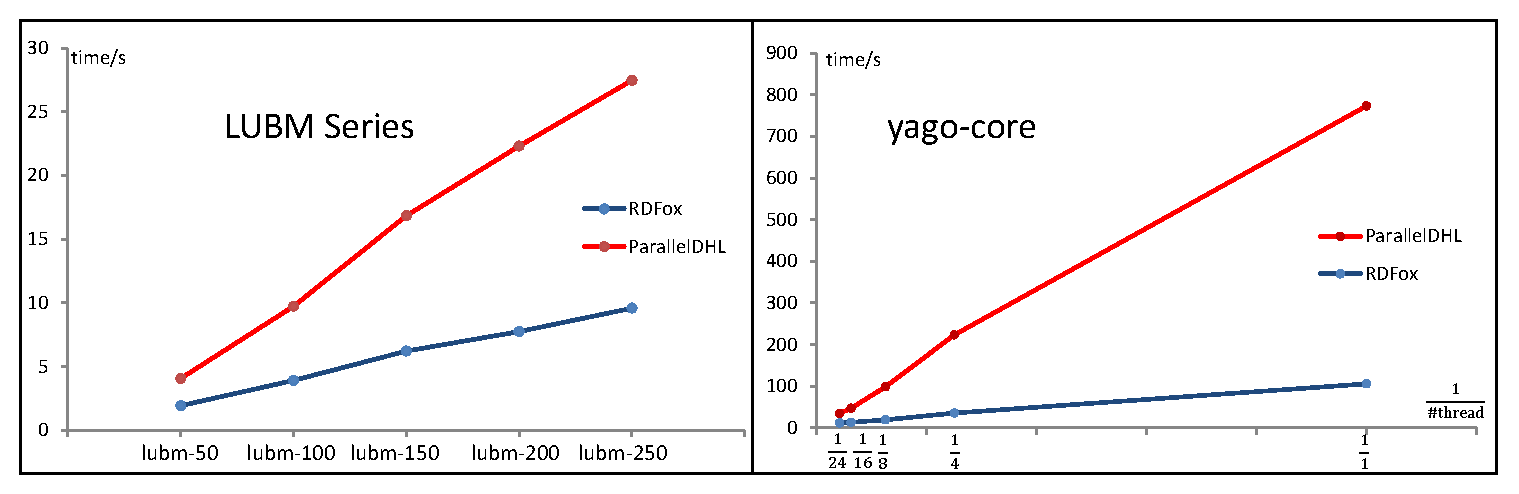
\includegraphics[width=1\textwidth]{fig-reasoningtime.eps}
\caption{(left) the reasoning times over the LUBM ontologies; (right) the reasoning times over yago-core.}
\label{fig:reasoningtime}
\end{center}
\end{figure}

From Table~\ref{tab:result}, we can see that for lubm-50 these two systems perform equally well.
For the other ontologies, ParallelDHL is comparable to RDFox with several threads being allocated.
For lubm-250 and yago-core, ParallelDHL delays obviously when only one thread is allocated.
The reason is that the computation of the relation $S_{\textit{\!\tiny rch}}$ occupies a large amount of time. When
more threads are allocated, ParallelDHL has a better efficiency.
Although ParallelDHL is not such optimized as RDFox, it also shows the scalability.
From the two line graphs in Figure~\ref{fig:reasoningtime},
we can see a linear trend of the reasoning times of both RDFox and ParallelDHL.
This also indicates that ParallelDHL will finish the materialization tasks on the test ontologies
in a shorter period of time with more threads being allocated.

\subsection{The Discussion of The Depths of Materialization Graphs}

From the complexity analysis for Algorithm~$\mathsf{A}_{bsc}$, we have that the computing time of
Algorithm~$\mathsf{A}_{bsc}$ depends on the number of iterations of \ref{alg1:updateG},
which equals to the depth of the constructed materialization graph (see the proof of Theorem~\ref{theorem:a1}).
Thus, the depth of the target materialization graph determines the computing time of
Algorithm~$\mathsf{A}_{bsc}$. This conclusion also applies to Algorithm~$\mathsf{A}_{opt}$
based on the analysis in Section~\ref{sec:opt}. In this part,
we discuss the influence of the depths of the materialization graphs
for the test ontologies.

\begin{figure}[htbp]
\begin{center}
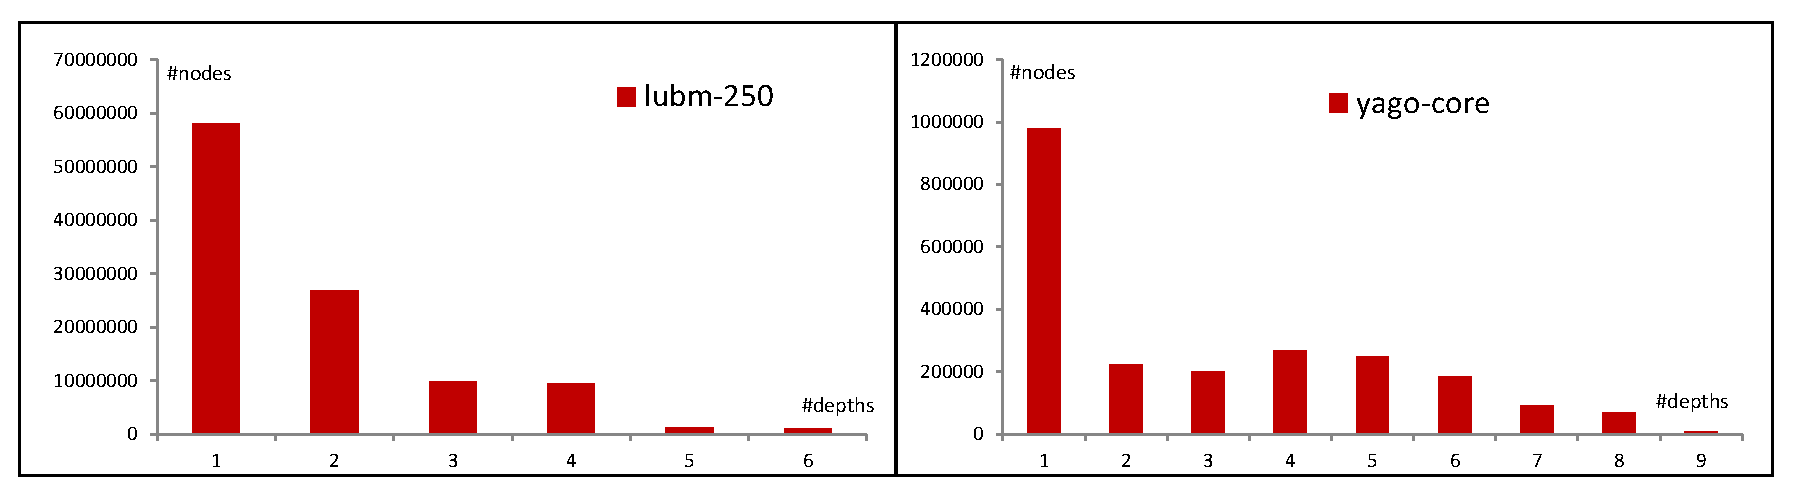
\includegraphics[width=1\textwidth]{fig-graphdepth.eps}
\caption{The statistics of the materialization graphs of lubm-250 (left) and yago-core (right).}
\label{fig:graphdepth}
\end{center}
\end{figure}

For the five test LUBM ontologies and the yago-core ontology, we record the total depth
of the materialization graph for each ontology and the number of nodes in different depths.
We have that all of the LUBM ontologies have the depth of 6 for their
materialization graphs, while the materialization graph of the yago-core ontology
has the depth of 9.
We use the histograms to graphically display the detailed data of lubm-250 and yago-core in Figure~\ref{fig:graphdepth},
where for each of the two histograms
the abscissa records the depths from the bottom of a materialization graph to the top,
the histograms denote the amount of nodes in each depth.

From the above results, we can find that the graph depths are far less than
the sizes of the input ontologies. Since the graph depth determines the computing
time of Algorithm~$\mathsf{A}_{bsc}$ and Algorithm~$\mathsf{A}_{opt}$ as discussed
at the beginning of this part,
the test ontologies should be materialized efficiently using these two algorithms.
The obvious difference of the reasoning times of the test ontologies is due to the limited memory space and the fixed number
of processors and the inapplicability of the parallel assumption given in Section~\ref{sec:alg-bsc}.
This results in that the computing
time of ParallelDHL does not depend only on the number of iterations of \ref{alg4:updateG}
of Algorithm~$\mathsf{A}_{prc}$ as analyzed in Section~\ref{sec:practicalAlg}.
It depends on several factors: the balancing of workload, the delay of some processors,
the I/O blocking, etc. Since these issues are not our focus, we do not analyze them in this work.
On the other hand, the results of the graph depths
indicate that we can further improve the performance of the materialization task by using more
memory space and more processors.



%%% Local Variables:
%%% mode: latex
%%% TeX-master: "parallel-tractability-J"
%%% End:
